\documentclass[14 pt]{article}
\usepackage[english]{babel}
\usepackage[utf8]{inputenc}
\usepackage[pdftex]{graphicx}

\newcommand*{\TitleFont}{%
	\usefont{\encodingdefault}
{\rmdefault}{i}{n}%
	\fontsize{48}{20}%
	\selectfont}

\title{\TitleFont Tron}
\author{Ch.Y.N.S.Avinash Karthik, N.N.Chaitanya, Aman Bhatia}
\date{March 2015}

\usepackage{natbib}
\usepackage{graphicx}

\begin{document}

\maketitle

\section{Introduction}
There are many games being introduced for entertaining computer users. Nowadays simple multiplayer games are much more popular than complicated single player games. We decided to create the game "Tron".\\

\begin{figure}[h!]
\centering
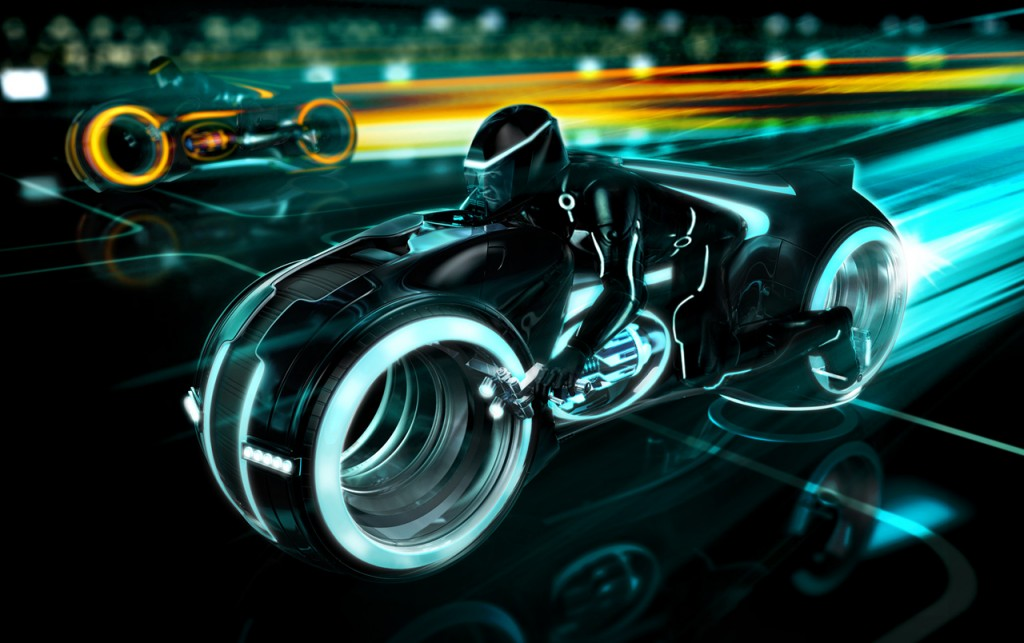
\includegraphics[width =100 mm]{2.jpg}
\footnote{Image Sources : Tron image is taken from Google-Images.}\\
\caption{Tron Movie Picture}
%\label{fig:univerise}
\end{figure}

\section{Motivation For The Game}
    Our motivation to create this game is from the movie "Tron Legacy". The movie had a very simple but attractive concept for a multiplayer game and hence we decided to implement this game.\\

\section{Gameplay}
    Each player is associated with a color. All the players start at some random positions and their path is captured or colored from their respective starting position with their respective color. Whenever a player crosses or even touches any colored path, then he explodes i.e. his game is over. The one who lasts longer in the game wins. Hence ranking will be decided by the time of survival of players. The number of players can be from 1 to 6.\\\\
    Various strategies can be used by the players to corner the players of the rival team and eliminate them.\\\\
    In addition, there is also an option to have players controlled by the computer so that when less number of users can play with some virtual players.\\


\section{Overall Design}
    The project aims at creating a user-appealing and elegant game application of Tron. There are four main components for making this multiplayer game. They are - Game Logic, Networking, GUI and Artificial Intelligence.\\

\begin{figure}[h!]
\centering
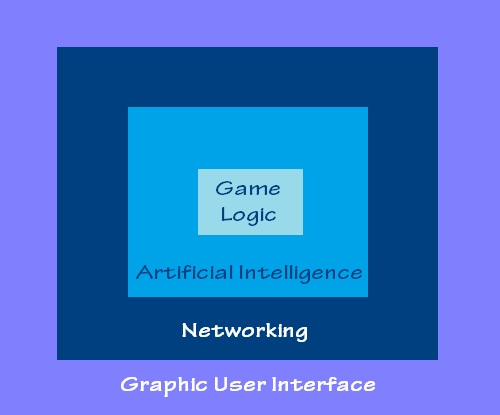
\includegraphics[width =100 mm]{5.jpg}
\footnote{Image Sources : Overall Design image is taken from Google-Images.}\\
\caption{Overall Design}
%\label{fig:univerise}
\end{figure}

\subsection{Game Logic}
    This is the main part of the game. It has the basic code of each player i.e. colour, path covered (walls) and velocity direction. In addition, it also has the information of players who are connected in the game.\\

\subsection{Networking}
    When the game is first created by a host, the initial game state is transmitted by the host to all the computers which connect to it. Then the game starts and each computer starts simulating all the bikes using the game logic and artificial intelligence. When a player changes the game state in his computer using inputs, the same command is sent to all the other computers. When each of the other computers receives this command, they execute this command in their simulations to appropriately change their game states. This ensures that all computers are in the same game state as long as the network is functioning properly.\\
    
\subsection{GUI}
    Every game gets popular if and only if it's graphics are appealing. All the graphics part including user friendly controls and options play a vital role in the success of a game. All the graphics like room, walls and bike designs including some other menu options are covered in GUI part.\\
    
\subsection{Artificial Intelligence}
    AI is used to control the computer controlled players. For a basic example of this, let's consider a computer player approaching a wall. Then the computer player should realize that he should turn so that he will not collide and lose the match. Hence for less number of players, the more efficient AI is, the more interesting the game would be.\\

\section{Implementation of Features}
\subsection{Networking}
    Networking is the backbone of multiplayer game. The more efficient the networking is, the more controlled the game would be.\\

\subsubsection{Content Of The Messages}
    If a player changes the game state in his computer, the command issued by this user is sent to all the other users. The content of the messages would therefore be the inputs given by the user to his own computer. In our case this would mean that information on which key or mouse button was pressed would have to transmitted.\\

\subsubsection{Choice Of Networking Protocol}
    Since we need to only transmit the key and mouse button presses, the rate at which messages have to be exchanged is very less. However, the order in which messages are exchanged is very important as it decides the changes in game state. Even a small change in the order of messages would jeopardise the synchronisation of the game states in all the computers. The TCP protocol of networking caters effectively to our need of network precision.\\

\begin{figure}[h!]
\centering
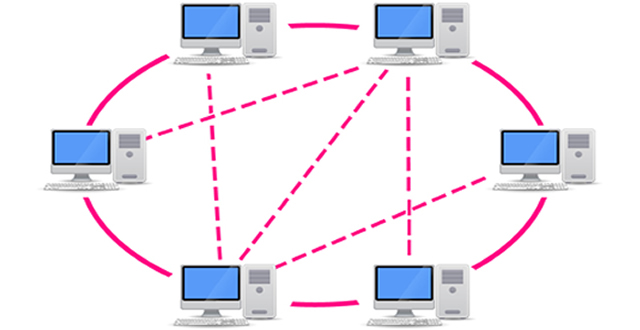
\includegraphics[width =100 mm]{4.jpg}
\footnote{Image Sources : Networking image is taken from Google-Images.}\\
\caption{Networking}
%\label{fig:univerise}
\end{figure}

\subsubsection{Choice Of Networking Method}
    In a standard server-client model of networking, the server is a very important component which decides the games state on it's own. However if the server goes down in the middle of the game, the games of all the other players would stop. In order to get around this, we plan to use peer-to-peer method of connection.\\

\subsubsection{Implementation of Peer-to-Peer Connection}
    A computer would initially act as a temporary server and create a game state depending on the number of players. When the required number of connections are made to the server, it messages all the information received to all the other computers. These computers now proceed to establish connections among themselves. After creation of these connections, the temporary server loses it's special status and becomes a normal peer like all the other computers.\\\\
    The game starts and any commands given by a user on a computer are transmitted to the other computers through their respective connections. The computer also waits to receive messages on each of the connections.\\
\subsubsection{Problems Encountered In Networking}
    One of the critical and difficult problems in networking is the network latency. The computer having the greatest latency decides how the game state evolves. The lag in network transmission results in a lag in the game state evolution.\\\\
    There would be no problem in all the cases where no player is eliminated from the game. This is because in this case each computer has to wait for messages from the computer simulating it's bike. It would not have to correct any of it's decision it takes on the bikes that is not owned by the player on that computer. In this case the state prediction by each computer would either be correct or would be correctable without visible effect in case it is wrong.\\\\
    Consider the following situation. Two players are playing the game and Player-1 is in a situation which decides whether he is eliminated from the game or not. The decision taken by Computer-2 on the bike of Player-1 is critical in this situation because in case the decision is wrong, the correction of the decision would result in visible effects.\\

\subsubsection{Solving The Problems}
    To tackle the network lag problem, the following convention can be followed in the game logic. The fate of each bike is decided by the computer on which the bike's player is playing. Thus, if Player-1's bike is in the above said situation, then Computer-2 waits for a message from Computer-1. Based on the inputs from Player-1, Computer-1 decides if Bike-1 stays in the game or not and continues simulating the bike. It also sends the decision to Computer-2 which then continues it's own simulation by factoring in the decision.\\


\subsection{Graphical User Interface(GUI)}
    We will try to make the GUI similar to what it is shown in the original movie. Basic outline of the Graphical User Interface part is as follows -\\

\subsubsection{StartUp Screen}
    When the program starts, firstly user has to choose between offline and online mode. User plays with the computer in the offline environment and with other players in the latter. Currently, we are thinking of making an application where game starts right away. Later if time permits, we will provide features like selection of bike, color of bike, environment options etc.\\
    
\subsubsection{Offline Mode}
    Offline gaming mode is very straight forward. The user plays against the computer i.e. their would be a one-on-one between the user and a single computer player.\\

\begin{figure}[h!]
\centering
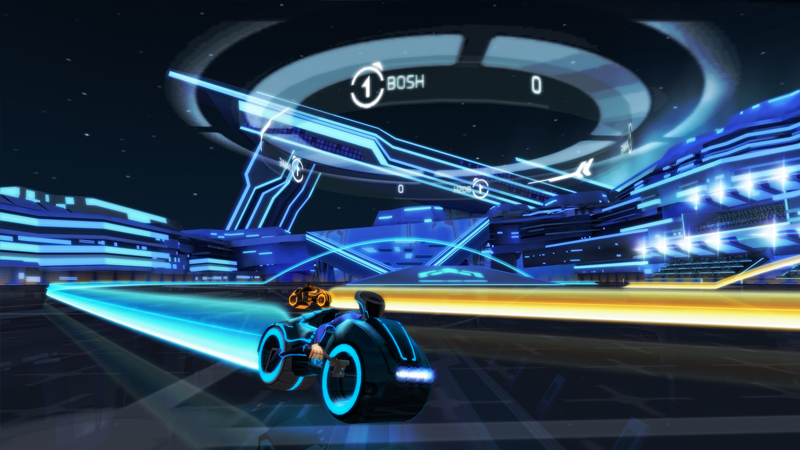
\includegraphics[width =120 mm]{1.jpg}
\footnote{Image Sources : Dropbox image is taken from Google-Images.}\\
\caption{GUI}
%\label{fig:univerise}
\end{figure}

\subsubsection{Online Mode}
    In online gaming mode, user is again prompted to fill details of the server i.e. user is supposed to provide host name and port name of the server. If the program is unable to connect to the server, the user is again prompted to fill the details or go back. If the connection is successful, then user is placed in the game arena to play with his friends.\\
    
\subsubsection{Game arena and Bikes}
    As we are trying to give the feel of the original movie, Game arena is basically a room of dark electric blue color. Same is the color of the walls. Bikes would be of blue, red, green, yellow, purple and white colors. As each bike goes on, the bike leaves a wall of the same color behind it. All the players are supposed to dodge these walls and the walls of the room.\\
    
\subsubsection{Game controls and Scoring}
    The game controls are quite simple. The user can just go left or right. So, we will use left arrow and right arrow for it. For scoring, the one who lasts in the game longest wins the game.\\
    
\subsubsection{Libraries and Packages}
    We will use Qt with openGL for this project. We choose Qt because if we feel the need of adding fascinating User Controls, then we can use Qt and integrate our openGL functions with it.\\
    
    
\subsection{Artificial Intelligence}
    Artificial Intelligence means the theory and development of computer systems able to perform tasks normally requiring human intelligence, such as visual perception, speech recognition, decision-making, and translation between languages.\\\\
    In every game, artificial intelligence plays a very important role. The more efficient the artificial intelligence is, the more interesting the game would be.\\\\
    In this game, artificial intelligence is used to control the computer controlled players. For computer controlled players, artificial intelligence is further divided into two parts - Attacking and Defencing.


\subsubsection{Attacking}
    Attacking in this game means doing a move so that the player who attacks can trap another player and hence destroy him. By this the attacking player can gain points.\\\\
    The main kind of attacking in this game is that when a player follows some other player parallely and the distance between the two players is appropriate, then the one who is been followed can attack the following player by making a 'U' kind of wall around the following player. This trap is successful almost everytime.\\\\
    There is also a small kind of attack in this game. When a player enters 3 sided surrounded junction, then some other player can close the fourth side of the junction by passing through that 4th side so the his tail wall can cover that junction. Hence the player trapped inside the box will ultimately die.\\
    
\begin{figure}[h!]
\centering
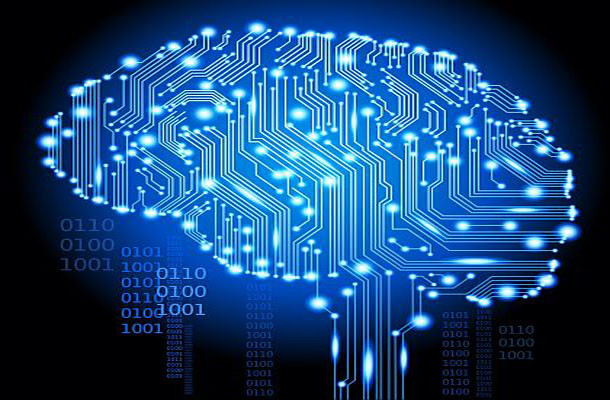
\includegraphics[width =100 mm]{3.jpg}
\footnote{Image Sources : Dropbox image is taken from Google-Images.}\\
\caption{Artificial Intellligence}
%\label{fig:univerise}
\end{figure}

\subsubsection{Defencing}
    Defencing in this game means being away from traps created by other players. Since the player who last for a longer time wins the game, the more defencive a player is, the more probability there will be for that player to win the game.\\\\
    The most basic defensive part is not colliding with the walls (both the actual walls or boundaries of the game and the walls created by other players). This can be easily done by taking a turn as the player gets closer to a wall.\\\\
    Taking appropriate turn is also a good defensive strategy. Hence the most basic intelligent way is to take a turn in the direction where the wall is some what at a greater distance so that he would not collide with the wall and also trapping probability will be less.\\
\subsubsection{Implementing these strategies}
    The above discussed strategies are implemented by using a simple state machine in c++. The transitions in the state machine should be unambiguous and should not have any bugs. Hence the more simple the machine is, the less probable the bugs to occur.\\\\
    Now coming to the transitions in the state machine, defence gets higher priority than attack because attacking without any backup leads to killing of the attacking player itself. Hence first the player tries to see whether he is in a good defensive position. If it is true, then he will see whether he is able to attack someone near him. If attacking is also not possible, then the player continues to move in that particular direction.\\\\
    Also to make the turns some what realistic, i.e turns to be unpredictable, a random turn can occur at any point if a player continues to move in a particular direction for sometime.\\\\

\section{Testing}
    The main components to test in this project are Artificial Intelligence, and the game logic. After making the final application, we can test basic artificial intelligence by just making to play two computer players. Advance AI i.e. all the cases handled for defence and attacking can be manually checked by creating appropriate game environment/situation. Also to take care of bugs, the application will be played as many times as possible so that the final submitted product has very minimal or no bugs. By running these test cases, the game logic will also be automatically tested because all the game logic bugs will be covered in the above mentioned test cases for AI.
%\bibliographystyle{plain}
%\bibliography{references}
\begin{center}
END OF DOCUMENT
\end{center}
\end{document}
